\documentclass[journal,12pt,twocolumn]{IEEEtran}
%
\usepackage{setspace}
\usepackage{gensymb}
%\doublespacing
\singlespacing

%\usepackage{graphicx}
%\usepackage{amssymb}
%\usepackage{relsize}
\usepackage[cmex10]{amsmath}
%\usepackage{amsthm}
%\interdisplaylinepenalty=2500
%\savesymbol{iint}
%\usepackage{txfonts}
%\restoresymbol{TXF}{iint}
%\usepackage{wasysym}
\usepackage{amsthm}
%\usepackage{iithtlc}
\usepackage{mathrsfs}
\usepackage{txfonts}
\usepackage{stfloats}
\usepackage{bm}
\usepackage{cite}
\usepackage{cases}
\usepackage{subfig}
%\usepackage{xtab}
\usepackage{longtable}
\usepackage{multirow}
%\usepackage{algorithm}
%\usepackage{algpseudocode}
\usepackage{enumitem}
\usepackage{mathtools}
\usepackage{tikz}
\usepackage{circuitikz}
\usepackage{verbatim}
\usepackage{tfrupee}
\usepackage[breaklinks=true]{hyperref}
%\usepackage{stmaryrd}
\usepackage{tkz-euclide} % loads  TikZ and tkz-base
\usetkzobj{all}
\usetikzlibrary{decorations.markings}
\usetikzlibrary{shapes.geometric}
\newif\iflabrev
\usepackage{listings}
    \usepackage{color}                                            %%
    \usepackage{array}                                            %%
    \usepackage{longtable}                                        %%
    \usepackage{calc}                                             %%
    \usepackage{multirow}                                         %%
    \usepackage{hhline}                                           %%
    \usepackage{ifthen}                                           %%
  %optionally (for landscape tables embedded in another document): %%
    \usepackage{lscape}     
\usepackage{multicol}
\usepackage{chngcntr}
%\usepackage{enumerate}

%\usepackage{wasysym}
%\newcounter{MYtempeqncnt}
\DeclareMathOperator*{\Res}{Res}
%\renewcommand{\baselinestretch}{2}
\renewcommand\thesection{\arabic{section}}
\renewcommand\thesubsection{\thesection.\arabic{subsection}}
\renewcommand\thesubsubsection{\thesubsection.\arabic{subsubsection}}

\renewcommand\thesectiondis{\arabic{section}}
\renewcommand\thesubsectiondis{\thesectiondis.\arabic{subsection}}
\renewcommand\thesubsubsectiondis{\thesubsectiondis.\arabic{subsubsection}}

% correct bad hyphenation here
\hyphenation{op-tical net-works semi-conduc-tor}
\def\inputGnumericTable{}                                 %%

\lstset{
%language=C,
frame=single, 
breaklines=true,
columns=fullflexible
}
%\lstset{
%language=tex,
%frame=single, 
%breaklines=true
%}

\begin{document}
%


\newtheorem{theorem}{Theorem}[section]
\newtheorem{problem}{Problem}
\newtheorem{proposition}{Proposition}[section]
\newtheorem{lemma}{Lemma}[section]
\newtheorem{corollary}[theorem]{Corollary}
\newtheorem{example}{Example}[section]
\newtheorem{definition}[problem]{Definition}
%\newtheorem{thm}{Theorem}[section] 
%\newtheorem{defn}[thm]{Definition}
%\newtheorem{algorithm}{Algorithm}[section]
%\newtheorem{cor}{Corollary}
\newcommand{\BEQA}{\begin{eqnarray}}
\newcommand{\EEQA}{\end{eqnarray}}
\newcommand{\define}{\stackrel{\triangle}{=}}
\bibliographystyle{IEEEtran}
%\bibliographystyle{ieeetr}
\providecommand{\mbf}{\mathbf}
\providecommand{\pr}[1]{\ensuremath{\Pr\left(#1\right)}}
\providecommand{\qfunc}[1]{\ensuremath{Q\left(#1\right)}}
\providecommand{\sbrak}[1]{\ensuremath{{}\left[#1\right]}}
\providecommand{\lsbrak}[1]{\ensuremath{{}\left[#1\right.}}
\providecommand{\rsbrak}[1]{\ensuremath{{}\left.#1\right]}}
\providecommand{\brak}[1]{\ensuremath{\left(#1\right)}}
\providecommand{\lbrak}[1]{\ensuremath{\left(#1\right.}}
\providecommand{\rbrak}[1]{\ensuremath{\left.#1\right)}}
\providecommand{\cbrak}[1]{\ensuremath{\left\{#1\right\}}}
\providecommand{\lcbrak}[1]{\ensuremath{\left\{#1\right.}}
\providecommand{\rcbrak}[1]{\ensuremath{\left.#1\right\}}}
\theoremstyle{remark}
\newtheorem{rem}{Remark}
\newcommand{\sgn}{\mathop{\mathrm{sgn}}}
\providecommand{\abs}[1]{\left\vert#1\right\vert}
\providecommand{\res}[1]{\Res\displaylimits_{#1}} 
\providecommand{\norm}[1]{\left\lVert#1\right\rVert}
%\providecommand{\norm}[1]{\lVert#1\rVert}
\providecommand{\mtx}[1]{\mathbf{#1}}
\providecommand{\mean}[1]{E\left[ #1 \right]}
\providecommand{\fourier}{\overset{\mathcal{F}}{ \rightleftharpoons}}
%\providecommand{\hilbert}{\overset{\mathcal{H}}{ \rightleftharpoons}}
\providecommand{\system}{\overset{\mathcal{H}}{ \longleftrightarrow}}
	%\newcommand{\solution}[2]{\textbf{Solution:}{#1}}
\newcommand{\solution}{\noindent \textbf{Solution: }}
\newcommand{\cosec}{\,\text{cosec}\,}
\providecommand{\dec}[2]{\ensuremath{\overset{#1}{\underset{#2}{\gtrless}}}}
\newcommand{\myvec}[1]{\ensuremath{\begin{pmatrix}#1\end{pmatrix}}}
\newcommand{\mydet}[1]{\ensuremath{\begin{vmatrix}#1\end{vmatrix}}}
%\numberwithin{equation}{section}
\numberwithin{equation}{subsection}
%\numberwithin{problem}{section}
%\numberwithin{definition}{section}
\makeatletter
\@addtoreset{figure}{problem}
\makeatother
\let\StandardTheFigure\thefigure
\let\vec\mathbf
%\renewcommand{\thefigure}{\theproblem.\arabic{figure}}
\renewcommand{\thefigure}{\theproblem}
%\setlist[enumerate,1]{before=\renewcommand\theequation{\theenumi.\arabic{equation}}
%\counterwithin{equation}{enumi}
%\renewcommand{\theequation}{\arabic{subsection}.\arabic{equation}}
\def\putbox#1#2#3{\makebox[0in][l]{\makebox[#1][l]{}\raisebox{\baselineskip}[0in][0in]{\raisebox{#2}[0in][0in]{#3}}}}
     \def\rightbox#1{\makebox[0in][r]{#1}}
     \def\centbox#1{\makebox[0in]{#1}}
     \def\topbox#1{\raisebox{-\baselineskip}[0in][0in]{#1}}
     \def\midbox#1{\raisebox{-0.5\baselineskip}[0in][0in]{#1}}
\vspace{3cm}
\title{
%	\logo{
Control Systems
%	}
}
\author{ G V V Sharma$^{*}$% <-this % stops a space
	\thanks{*The author is with the Department
		of Electrical Engineering, Indian Institute of Technology, Hyderabad
		502285 India e-mail:  gadepall@iith.ac.in. All content in this manual is released under GNU GPL.  Free and open source.}
	
}	
%\title{
%	\logo{Matrix Analysis through Octave}{\begin{center}\includegraphics[scale=.24]{tlc}\end{center}}{}{HAMDSP}
%}
% paper title
% can use linebreaks \\ within to get better formatting as desired
%\title{Matrix Analysis through Octave}
%
%
% author names and IEEE memberships
% note positions of commas and nonbreaking spaces ( ~ ) LaTeX will not break
% a structure at a ~ so this keeps an author's name from being broken across
% two lines.
% use \thanks{} to gain access to the first footnote area
% a separate \thanks must be used for each paragraph as LaTeX2e's \thanks
% was not built to handle multiple paragraphs
%
%\author{<-this % stops a space
%\thanks{}}
%}
% note the % following the last \IEEEmembership and also \thanks - 
% these prevent an unwanted space from occurring between the last author name
% and the end of the author line. i.e., if you had this:
% 
% \author{....lastname \thanks{...} \thanks{...} }
%                     ^------------^------------^----Do not want these spaces!
%
% a space would be appended to the last name and could cause every name on that
% line to be shifted left slightly. This is one of those "LaTeX things". For
% instance, "\textbf{A} \textbf{B}" will typeset as "A B" not "AB". To get
% "AB" then you have to do: "\textbf{A}\textbf{B}"
% \thanks is no different in this regard, so shield the last } of each \thanks
% that ends a line with a % and do not let a space in before the next \thanks.
% Spaces after \IEEEmembership other than the last one are OK (and needed) as
% you are supposed to have spaces between the names. For what it is worth,
% this is a minor point as most people would not even notice if the said evil
% space somehow managed to creep in.
% The paper headers
%\markboth{Journal of \LaTeX\ Class Files,~Vol.~6, No.~1, January~2007}%
%{Shell \MakeLowercase{\textit{et al.}}: Bare Demo of IEEEtran.cls for Journals}
% The only time the second header will appear is for the odd numbered pages
% after the title page when using the twoside option.
% 
% *** Note that you probably will NOT want to include the author's ***
% *** name in the headers of peer review papers.                   ***
% You can use \ifCLASSOPTIONpeerreview for conditional compilation here if
% you desire.
% If you want to put a publisher's ID mark on the page you can do it like
% this:
%\IEEEpubid{0000--0000/00\$00.00~\copyright~2007 IEEE}
% Remember, if you use this you must call \IEEEpubidadjcol in the second
% column for its text to clear the IEEEpubid mark.
% make the title area
\maketitle
\newpage
\tableofcontents
\bigskip
\renewcommand{\thefigure}{\theenumi}
\renewcommand{\thetable}{\theenumi}
%\renewcommand{\theequation}{\theenumi}
%\begin{abstract}
%%\boldmath
%In this letter, an algorithm for evaluating the exact analytical bit error rate  (BER)  for the piecewise linear (PL) combiner for  multiple relays is presented. Previous results were available only for upto three relays. The algorithm is unique in the sense that  the actual mathematical expressions, that are prohibitively large, need not be explicitly obtained. The diversity gain due to multiple relays is shown through plots of the analytical BER, well supported by simulations. 
%
%\end{abstract}
% IEEEtran.cls defaults to using nonbold math in the Abstract.
% This preserves the distinction between vectors and scalars. However,
% if the journal you are submitting to favors bold math in the abstract,
% then you can use LaTeX's standard command \boldmath at the very start
% of the abstract to achieve this. Many IEEE journals frown on math
% in the abstract anyway.
% Note that keywords are not normally used for peerreview papers.
%\begin{IEEEkeywords}
%Cooperative diversity, decode and forward, piecewise linear
%\end{IEEEkeywords}
% For peer review papers, you can put extra information on the cover
% page as needed:
% \ifCLASSOPTIONpeerreview
% \begin{center} \bfseries EDICS Category: 3-BBND \end{center}
% \fi
%
% For peerreview papers, this IEEEtran command inserts a page break and
% creates the second title. It will be ignored for other modes.
%\IEEEpeerreviewmaketitle
\begin{abstract}
This manual is an introduction to control systems based on GATE problems.Links to sample Python codes are available in the text.  
\end{abstract}
Download python codes using 
\begin{lstlisting}
svn co https://github.com/gadepall/school/trunk/control/codes
\end{lstlisting}
%\section{Mason's Gain Formula}
%\section{Bode Plot}
%\subsection{Introduction}
%\subsection{Example}
%\section{Second order System}
%\subsection{Damping}
%\subsection{Example}
%\section{Routh Hurwitz Criterion}
%\subsection{Routh Array}
%\subsection{Marginal Stability}
%\subsection{Stability}
%\input{./chapters/EE18BTECH11021.tex}
%\section{State-Space Model}
%\input{./chapters/ee18btech11004.tex}
%\subsection{Second Order System}
%\section{Nyquist Plot}
%\section{Phase Margin}
%\section{Gain Margin}
%\section{Compensators}
%\subsection{Phase Lead}
%\input{./chapters/EE18BTECH11021_2.tex}
%\section{Oscillator}
\section{Compensators}
\begin{enumerate}[label=\thesection.\arabic*.,ref=\thesection.\theenumi]
\numberwithin{equation}{enumi}

\item Why do we use compensators. \\
\solution In order to obtain the desired performance of the system, we use compensating networks.

\item What is the use of a Phase lead compensator. \\
\solution Phase lead compensator is used to increase the stability or speed of response of a system.

\item What is the use of phase lag compensator. \\
\solution Phase lag compensator lag compensator is used to reduce (but not eliminate) the steady-state error.

\item Write the general expression for the transfer function of a phase lead compensator. \\
\solution 
\begin{align}
    H(s) = \frac{(1+ \alpha s T)}{(1+T s)}
\end{align}
$\alpha$ is generally less than 1 for Phase lead compensator.

\item Find the frequency range in which phase introduced by the phase lead compensator reaches maximum \\
\solution  Transfer function can be rewritten as 
\begin{align}
    H(j\omega) = \frac{(1+ j \alpha \omega T)}{(1+j \omega T)}
\end{align}
Then phase introduced by transfer function is given by 
\begin{align}
    \phi = tan^{-1}(\alpha \omega T) - tan^{-1}(\omega T)
\end{align}
Upon differentiating
\begin{align}
    \frac{d\phi}{d\omega} = \frac{\alpha T}{1 + (\alpha \omega T)^2} - \frac{T}{1 + (\omega T)^2}
\end{align}
Equating it to zero to find the maximum
\begin{align}
    \frac{\alpha T}{1 + (\alpha \omega T)^2} = \frac{T}{1 + (\omega T)^2} \\
    \alpha(1 +(\omega T)^2) = 1 + (\omega \alpha T)^2 \\
    \alpha + \alpha(\omega T)^2 = 1 + (\omega \alpha T)^2 \\
    (\alpha - 1) = (\omega T)^2 \alpha(\alpha -1) \\
    (\omega)^2 = \frac{1}{(T^2) \alpha} \\ 
    \omega = \frac{1}{T \sqrt{\alpha}}
\end{align}
Clearly
\begin{align}
    \frac{1}{\alpha T} < \frac{1}{T \sqrt{\alpha}} < \frac{1}{T}
\end{align}
So the frequency range in which phase lead introduced by this compensator reaches maximum in 
\begin{align}
    \omega \epsilon (\frac{1}{\alpha T} , \frac{1}{T})    
\end{align}


\item Write the general expression for the transfer function of phase lag compensator. \\
\solution 
\begin{align}
    H(s) = \frac{1}{\beta}\frac{(1+ \beta s T)}{(1+T s)}
\end{align} 
$\beta$ is generally greater than 1 for Phase lead compensator.


\item
Write the general expression for the transfer function of a Phase lag-lead compensator. \\
\solution
The Transfer Function of the Phase lag-lead compensator is
\begin{align}
    H(s) = \frac{(1+ \alpha s T_1)(1+ \beta s T_2)}{(1+T_1 s)(1 + T_2 s)}
\end{align}
$\alpha$ and $\beta$ are generally chosen in such a way that
\begin{align}
    \alpha \beta = 1
\end{align}

It is to be noted that phase introduced by lag part is close to zero in the frequency range where lead part reaches maximum and vice versa.

\item Write the expression for phase introduced by phase lag-lead compensator. \\
\solution 
\begin{align}
    \phi = tan^{-1}(\frac{\omega T_1}{\beta}) + tan^{-1}( \beta \omega T_2) - tan^{-1}(\omega T_1) - tan^{-1}(\omega T_2)
\end{align}

\item Consider the Transfer function of a phase lag-lead compensator
\begin{align}
    C(s) = \frac{(1+\frac{s}{0.1})(1+\frac{s}{100})}{(1+\frac{s}{1})(1+\frac{s}{10})}
\end{align}
Find the frequency range in which the phase (lead) introduced by the compensator reaches the maximum \\ 
\solution 
Comparing the given Transfer function with with equation(1.7.1), we get $\alpha$ = 10, $T_1$ = 1, $\beta$ = 0.1, $T_2$ = 0.1.
Substituting these values in equation (1.8.1)
\begin{align}
    \phi = tan^{-1}(10\omega) + tan^{-1}(0.01\omega) - tan^{-1}(\omega) - tan^{-1}(0.1\omega)
\end{align}
As we are trying to find the range of frequencies in which Phase lead introduced by the compensator is maximum, the phase introduced by the lag part of compensator will be close to zero.
\begin{align}
    \phi = tan^{-1}(10 \omega ) - tan^{-1}(\omega )
\end{align}
This is similar to equation 1.5.2 and we already know that in this case $\phi$ is maximum for 
\begin{align}
    \omega \epsilon (0.1,1)
\end{align}

\item Verify using a python plot \\ 
\solution
\begin{lstlisting}
codes/EE18BTECH11044.py
\end{lstlisting}

\begin{figure}[h!]
\centering
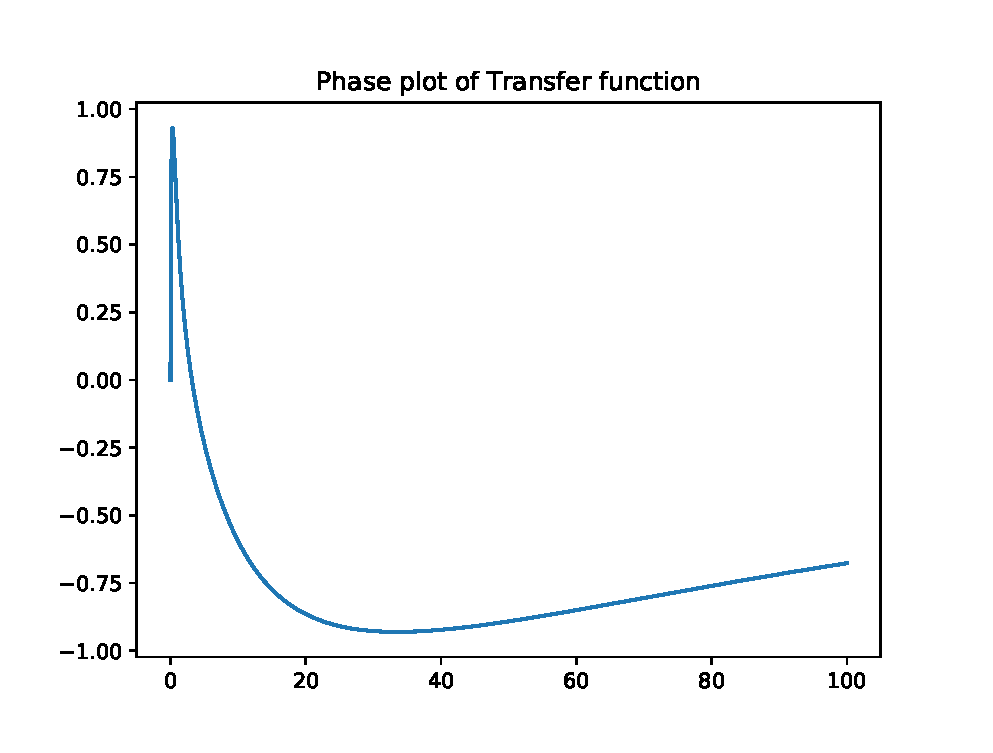
\includegraphics[width=\columnwidth]{figs/EE18BTECH11044.eps}
\end{figure}


\end{enumerate}

\end{document}
